$\mathcal{R} _{r, R} (a ) = \{ z \in \C \mid q < |z -a | < R\}$.

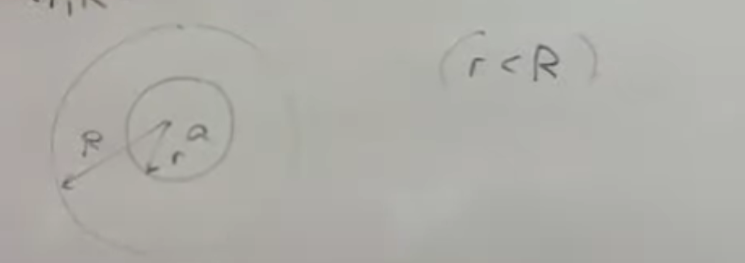
\includegraphics[scale=0.6]{img/convergence_ring_Laurent_series.png}

$a \in \C; f \in mathrm{Hal} \left(mathcal R _{r, R} (a)\right)$, где $-\infty \leqslant r < R \leqslant +\infty \implies \exists $ едиственный $(C_k)_{k\in \Z}\subset \C $:
\[\forall z \in \mathcal{R}_{r, R}(a),~~~~
f(z) = \sum_{k\in\Z} c_k (z 0 a )^k.
    \]

$c_k = \dfrac{1}{2\pi} \cdot \oint_{|z -a | \rho } \dfrac{f(z)}{(z - a) ^{k + 1}},~~~\rho \in (r, R) $.

\begin{definition}
    $a \in \overline{\C}$ называют изолированной особой точке $f(z)$, если $\exists$ окрестность $U(a)$:
    \[ f(z) \in \mathrm{Hol}(\overset{\cdot } {U} (a)). \]
\end{definition}
\begin{example}
\begin{enumerate}
    \item $f(z) = z$,~~~ $A = \{\infty  \}$.
    \item $f(z) = \overline{z}$,~~~ $ A = \O$ (все точки дифференцируемы).
    \item $f(z ) = \dfrac{1}{2} \left( z + \dfrac{1}{z} \right)$,~~~ $A = \{ 0, \infty\}$.
\end{enumerate}
\end{example}


\begin{definition}
    Пусть $a \in \overline{\C}$~--- и.о.т. $f(z)$. Тогда $a$ называется
    \begin{itemize}
        \item Полюсом $\iff \exists \lim_{z\to a} f(z) = \infty$.
        \item Существенно особой $\iff \not \exists \lim_{z\to a} f(z)$.
    \end{itemize}
\end{definition}

\begin{example}
\begin{enumerate}
    \item $f(z) = z$,~~~ $A = \{\infty  \}$, $\infty$~--- полюс.
    \item $f(z) = \dfrac{1}{2} \left( z + \dfrac{1}{z} \right)$,~~~ $A = \{ 0, \infty\}$, $0$ и $\infty$~--- полюсы.
    \item $f(z) = e^z$, ~~~ $A = \{\infty\}$,~~~ $\infty$~--- существенно особая точка.
\end{enumerate}
\end{example}

\begin{statement}
    Пусть $a\in \C, ~~~a$~--- и.о.т. $f(z)$. $\exists R~: f \in \mathrm{Hol}\left( \overset{\cdot}{B}_R (a) \right)$.\\
    Пусть $f (z) = \underbrace{\sum_{k = 0}^{+\infty } c_k (z - a)^k}_{\text{регулярная часть}} + \underbrace{\sum_{k \in -\N} c_k (z - a)^k}_{\text{главная часть лорановского разложения } f(z) \text{при} z \to a}$ ~~$\forall z \in \overset{\cdot}B_R (a)$.
\end{statement}

\begin{example}
    $f (z) = \dfrac{1}{1- z}$.

    В точке $z = 0$. Так как $f(z ) \in \mathrm{Hol} \left(B_1 (0) \right) \implies f(z) = \sum_{k = 0}^ \infty z^{k},~~~\forall z \in z \in B_1 (0)$.  Регулярная часть есть, а главная отсутствует.

    В точке $z = 1$. $f(z) = (-1) (z - 1)^{-1}$~--- главная часть.

    $z$ в окрестности $\infty$ $\dfrac{1}{1 - z } = \left( \dfrac{-1}{z} \right) \cdot \dfrac{1 }{ 1 - \dfrac{1}{z}} = \left(-1 \dfrac{1}{z} \right) \cdot \sum_{k=0}^\infty \left( \dfrac{1}{z} \right)^k$. Все регулярная часть, главная отсутствует.
\end{example}

\begin{statement}[Характеристика изолированных особых точек в терминах Лорановского разложения]

Пусть $a \in \overline{\C}$, ~~~$a$~--- и.о.т. $f(z)$. Тогда
\begin{enumerate}
    \item $a$~--- устранимая $\iff \exists $ окрестность $U(a)~:~ f \big|_{\overset{\cdot}{U} (a)}$~--- ограниченная $\iff$ главная часть лорановского разложения отстутствует.
    \item $a$~--- полюс $\iff $ главная часть лорановского разложения $f(z)$ в окрестности $a$ содержит конечное число членов.
    \item $a$~--- существенно устранимая $\iff$ главная часть лорановского разложения $f(z)$ содержит бесконечное число слогаемых.
\end{enumerate}
\end{statement}

Неравенство Коши ~:~$f(z) = \sum_{k \in \Z} c_k (z - a)^k, ~~~a \in \C$. $M_r = \sup_{z ~:~ |z - a | = r} |f| $,~~~ $ |c_k| \leqslant \dfrac{M_r}{r^k}$, $\forall k \in \Z$.

\begin{proof}
    ...
\end{proof}


\begin{note}
    Если $a \in \C$~--- и.о.т., то $\exists A~:~ \tl f (z) = \begin{cases}
        f(z),~~ z \neq a\\ A.
    \end{cases} \in \mathrm{Hol } (U(A))$.

    $f (z) = \sum_{k=0}^\infty c_k (z - a)^k$ в проколотой окрестности $a$.

    Проще говоря, можно исправить функцию в плохих точках и она станет хорошей.
\end{note}

\begin{example}
    $f(z) = \frac{sin z}{z} \in \mathrm{Hol}\left( \R \setminus \O  \right) $


    $f(z) = \frac{1}{z}\cdot \left( z - \frac{z^3}{3!}  + \frac{z^5}{5!} - \ldots \right) = 1 - \frac{z^2}{3!} + \frac{z^4}{5!} - \ldots$ -- сходится всюду в $\C$.
    Значит это продолжение функции $\frac{sin z}{z}$
\end{example}

\begin{note}
    [Отступление]

    \begin{lemma}
        [О кратности нуля]

        $f(z)\in \mathrm{Hol}\left( B_k(a) \right) , a\in \C, R>0$

        $f(a) = 0$ Тогда $\exists N\in \N : f(z) = (z-a)^N\cdot g(z)$, где $g(z)\in \mathrm{Hol}(B_k(a)), g(a)\neq 0 \implies f(z) \sim A \cdot (z-a)^N$, где $A = g(a)$
    \end{lemma}

    $f(z) = \sum_{k=0}^{\infty} c_k(z-a)^k$ в окрестности точки $a$, $c_0 = 0$
\end{note}

% эта часть куда идёт?.............

\begin{note}
    Если точка $a\in \C$ -- полюс, то $\sphericalangle g(z) = \frac{1}{f(z)}\to 0, z\to a$,
    $a$ -- устранимая для $g(z) \implies g(z) = (z-a)^N \cdot \tl g(z)\quad \tl g(a) \neq 0, \tl g\in \mathrm{Hol}(\text{окрестности т.} a)$

    \begin{align*}
        f &= \frac{1}{g} = \frac{1}{(z-a)^N} \frac{1}{\tl g(z)}\\
        &= \frac{1}{(z-a)^N} \cdot \left( \sum_{k=0}^{\infty} b_k(z-a)^k \right)  \\
        &= \frac{b_0}{(z-a)^N} + \frac{b_1}{(z-a)^{N-1}} + \ldots \\
    .\end{align*}
\end{note}

\begin{definition}
    $\sqsupset  a\in \C$ -- полюс для $f(z), N\in \N $

    $a$ -- полюс порядка $N$ для $f(z) \iff f(a) \sim \frac{C}{(z-a)^N} \left( \iff f(z) = \frac{g(z)}{(z-a)^n} \text{ где } g(z) \text{голоморфна в некоторой окрестности точка a функция}, g(a)\neq 0\right) $

    Для бесконечных точекрассматриваем $g(w) = \frac{1}{f(w)}$
\end{definition}

\begin{note}
    Любой полюс обладает порядком.
\end{note}

\begin{example}
    \begin{enumerate}
        \item $f(z) = \dfrac{1}{2 } \cdot \left( z + \dfrac{1}{z} \right)$. Полюс $0$ имеет порядок 1, полюс $\infty$ имеет порядок 1. Полюсы с порядком 1 называют \textbf{простыми}.
        \item $f(z) = \frac{\cos z - 1}{z^2} = \frac{-\frac{z^2}{2} + \frac{z^4}{4!} - \ldots}{z^3} = - \frac{1}{2z} + \ldots$. $0$ -- простой полюс (порядок 1), $\infty $ -- существенно особая.

        \item $f(z) = \tg z$. $\left\{ \frac{\pi}{2} + \pi k \right\}_{k\in \Z }$

        $\tg z = \frac{\sin z}{\cos z} \sim \frac{}{ \frac{\pi}{2} - z}\quad z = \frac{\pi}{2}$.  $\implies $ эти точки простые особые. $\infty $ -- не изолированная особая.
    \end{enumerate}
\end{example}

\begin{note}
    Почему может быть полезно знать какие особенности у функции в конкретной точке?
\end{note}

\begin{definition}
    $\sqsupset a\in \tl \C, a$ -- изолированная особая точка $f(z)$

    \[
    \res_a f = \begin{cases}
        c_{-1}&, \text{коэффициент в Лорановском разложении} f(z) \text{в окрестности точки} a\in \C\\
        -C_{-1}&, \text{коэффициент в Лорановском разложении} f(z) \text{в окрестности} \infty , a=\infty \\
    \end{cases}
    .\]
\end{definition}

\begin{example}
    \begin{enumerate}
        \item $f(z) = \frac{1}{2}(z + \frac{1}{z})\quad \res_0f = \frac{1}{2}, \res_{\infty }f = -\frac{1}{2}$
        \item $f(z) = \frac{1}{z^2 - 1} = \frac{1}{(z-1)(z+1)} = \frac{\frac{1}{2}}{z - 1} - \frac{\frac{1}{2}}{z+1}$

        $\res_1f = \res_1 \frac{\frac{1}{2}}{z - 1} = \frac{1}{2}\quad \res_{-1}f = -1\quad \res_{\infty }f = 0$, т.к. $f$ -- чётная
    \end{enumerate}
\end{example}

\begin{note}
    Чем хороши вычеты?
\end{note}

$c_k$ -- коэффициенты лорановского разложения в окрестности точки $a$, $f\in \mathrm{Hol}(B_R^\circ(a))$

\[
    c_k = \frac{1}{2\pi i} \oint _{|z+a| = \rho} \frac{f(z)}{(z-a)^{k+1}}dz\quad \rho\in(0,R)
.\]

$\res_af = c_{-1} = \frac{1}{2\pi i} \oint _{|z-a| = \rho}f(z)dz$

\begin{theorem}
    [Коши о вычетах]

    Пусть $O$ -- кусочно-гладкая область в $\tl \C$

    $A$ -- конечное множество, $A\subseteq O, f\in \mathrm{Hol}\left( \tl O \setminus A \right) $ Тогда:
    \[
    \int_{\partial O}f(z)dz = 2\pi i \sum_{a\in A}\res_a f = 2\pi i \sum_{z\in O}\res_zf
    .\]
\end{theorem}

\begin{theorem}
    [о полной сумме вычетов]


    $\sqsupset A\ni \infty , A\subseteq \tl \C, A$ -- конечно

    $\sqsupset f\in \mathrm{Hol}\left( \C \setminus A \right) $ Тогда:

    \[
    \sum_{a\in A}\res_af = \sum_{z\in \tl \C}\res_zf = 0
    .\]
\end{theorem}
\begin{proof}
    $\sqsupset A_0 = A \setminus \{\infty \}$

    Т.к. $A_0$ -- конечно, то $\exists B_R(0) \supset A_0$

    \begin{align*}
        \oint_{|z| = R} f(z)dz &= \left( \sum_{a\in A_0} \res_af \right) \cdot 2\pi i  \\
        &= \left( -\res_{\infty }\cdot 2\pi i \right)  \\
    .\end{align*}
\end{proof}

Приёмы вычсления вычетов ($a$ -- изолированная особая точка $f(z)$):
\begin{enumerate}
    \item $a$ -- устарнимая особая точка.
    \begin{enumerate}
        \item $a\in \C \implies \res_a f = 0$
        \item $a = \infty \quad f(z) = C_0 + \frac{C_1}{z} + \frac{C_2}{z^2} + \ldots$

        $\lim_{z \to \infty} f(z) = C_0$

        $\lim_{z \to \infty} z\left( f(\infty ) - f(z) \right) = \res_{\infty }f  $
    \end{enumerate}
    \item $a\in \C$ -- полюс. Тогда:
    $f(z) = \frac{C_{-N}}{(z-a)^N} + \ldots + \frac{C_{-1}}{(z-a)} + C_0 + C_1(z-a) + \ldots$

    $\res_af = \frac{1}{(N+1)!} \left( z_0 a^N f(z) \right) ^{(N-1)}_{z=a}$

    Если полюс простой, то $\res_af = \lim_{z \to a} f(z)(z-a)$

    Частный случай: $f(z) = \frac{\varphi(z)}{\psi(z)}, \varphi, \psi\in \mathrm{Hol}, \varphi(a) \neq 0, \psi(a) = 0, \p \psi(a) \neq 0$

    $\res_af = \lim_{z \to a} \frac{\varphi(z)}{\psi(z)}(z-a) = \lim_{z \to a} \frac{\varphi(z)}{\frac{\psi(z) - \psi(a)}{z - a}} = \frac{\varphi(a)}{\p\psi(a)}$

    \[
    \res_af = \frac{\varphi(a)}{\p\psi(a)}
    .\]
    \item Теорема о полной сумме вычетов.
    \item Если $f(z)$ чётная функция, то $\res_af = - \res_{-a}f$, в частности $\res_0 = 0 = \res_{\infty }$
    \item Если $f(z)$ нечётная, то $\res_af = \res_{-a}f$
\end{enumerate}

\begin{example}
    \begin{enumerate}
        \item $\int_{|z-1| = 1} \frac{dz}{z^4 +1}$

        $z^4 = -1$

        $z_1, z_4$ -- простые полюсы. $\res_{z_1}f = \frac{1}{4z_1^3} = \frac{z_1}{4z_1^4}  = - \frac{z_1}{4}$

        $\res_{z_2}f = -\frac{z_2}{4}$
        \begin{align*}
            \int_{|z-1| = 1} \frac{dz}{z^4 +1} &= 2\pi i\left( \res_{z_1} f + \res_{z_4} f \right)  \\
            &= -\frac{\pi i}{2}(z_1 + z_4) \\
            &= - \frac{\pi i}{2}\sqrt{2}  \\
        .\end{align*}
    \end{enumerate}
\end{example}



Приложение теоремы о вычетах к вычислению определённых и несобственных интегралов.
\begin{enumerate}
    \item $\int_{-\pi}^{\pi} R(\cos\varphi, \sin\varphi)d\varphi = \oint_{|z| = 1} R\left( \frac{z + \frac{1}{z}}{2}, \frac{z - \frac{1}{z}}{2} \right) \frac{dz}{iz} $

    \begin{align*}
        z = e^{i\varphi}\\
        \frac{z + \frac{1}{2}}{2} = \frac{e^{iz} + e^{-iz}}{2} = \cos z\\
        dz = de^{i\varphi} = i e^{i\varphi} d \varphi = i z d \varphi.
    \end{align*}
    \begin{example}

        $z^2+6z+1 = 0$

        $z_{12} = -2\pm \sqrt{9-1} = -3\pm 2\sqrt{2}  $

        $z_1z_2 = 1$ (по теореме Виета, о которой полезно помнить)

        $|z_1| = \frac{1}{|z_2|}$

        $z_1 $ -- полюс второго порядка


        \begin{align*}
            \int_{-\pi}^{\pi}\frac{\cos \varphi + 2}{\left( \cos \varphi +3 \right) ^2} d\varphi = \oint_{|z| = 1}\frac{\frac{z + \frac{1}{z}}{2} + 2}{\left(  \frac{z + \frac{1}{z}}{2} + 3 \right) ^3}\\
            &= \frac{2}{i}\int_{|z| = 1} \frac{z^4 + 4z + 1}{\left( z^2 + 6z + 1 \right)^2 }dz \\
            &= \frac{2}{i}2\pi i \cdot \res_{z_1}f(z) \\
            \res_{z_1} f &= \frac{1}{(N-1)!} (f(z)(z-a)^N)^{(N-1)}_{z=a} \\
            &= \p{(f(z)(z-1)^2)}\mid_{z=z_1} \\
            &= \frac{z^2+4z+1}{(z-z_2)^2}\mid_{z=z_1}\\
            &= \left( \frac{2z+4}{(z-z_2)^2} - 2 \frac{z^2 + 4z+1}{(z-z_2)^3} \right)\mid_{z = z_1} = \ldots.\end{align*}
    \end{example}
    \item Несобтсвенный интеграл $\int_{-\infty }^{\infty } f\left( x \right) dx$
    $f(x)$ допускает аналитическое продолжение в $\C \setminus A, A$ -- конечное множество особыз точек, $A \cap \R = \O $

    $\sup_{|z| = R} |f(z)| = o(\frac{1}{R})\quad R\to +\infty $

    Тогда:
    \[
        \int_{-\infty }^{\infty }f\left( x \right) dx = 2\pi i \sum_{z:\Im z >0}\res_z f
    .\]

    Мы можем рассмотреть семейство полукругов и брать интегралы по их контурам.

    $\int_{C_R}f(z)dz = 2\pi i \sum_{\substack{z:\Im z> 0\\ |z|< R}} \res_z f 2\pi i \sum_{z: \Im z > 0}\res_zf$

    $ = \int_{-R}^R f(z) dz + \int_{\substack{|z| = R\\ \Im z \geqslant 0}} f(z)dz \to \int_{-\infty }^{\infty }d(x)dx + 0$

    \begin{example}

        особые точки: $z^1 + 1=0;z^4 + 4 = 4\qquad z = \pm i\;z = \pm 2i\quad |z| = R$

        $|f(z)| = \frac{1}{|z^1 + 1| |z^2 + 4|}$
        \begin{align*}
            \int_0^{\infty } \frac{dx}{(x^2 + 1)(x^2 + 4)} = \frac{1}{2}\int_{-\infty }^{\infty } \frac{dx}{(x^2 + 1) (x^4 +4)}
        .\end{align*}
    \end{example}
\end{enumerate}

$M(R) = \sup_{|z| = R}\sup |f(z)| = o\left(\dfrac 1 R \right), R\to +\infty$ --- условие на применение формулы для несобственного интеграла

%% строчка
